\chapter{Anhang}

	\section{Klassendiagramm}
	
	% \clearpage
	% %%% -----------------------------------------------
	% \KOMAoptions{paper=a3,paper=landscape}
	% %%% -----------------------------------------------
	% \areaset{\dimexpr \textwidth+.5\paperwidth}{\textheight}
	% \noindent\begin{minipage}{\textwidth}
	%     \rule{\textwidth}{\dimexpr\textheight-3\baselineskip\relax}
	%     \captionof{figure}{Eine ziemlich breite Abbildung}
	% \end{minipage}
	
	% %
\includepdf[noautoscale=true, fitpaper=true,pagecommand={\rhead{\includegraphics[height=1cm]{logo.png}}\lfoot{}\cfoot{}\rfoot{\thepage}}]{diagrams/test.pdf}
	
	% \clearpage
	% \KOMAoptions{paper=a4,paper=portrait}
	% \areaset{\dimexpr \textwidth-\paperwidth}{\textheight}
	
	% wieder a4
	
	%%oder
	\getlength{\paperwidth}\\
	\getlength{\paperheight}\\
	\getlength{\pdfpageheight}\\
	\getlength{\pdfpagewidth}\\
	\getlength{\headwidth}\\
	\getlength{\footskip}\\
	\getlength{\textwidth}\\
	\getlength{\textheight}\\
	\getlength{\vsize}\\
	\getlength{\hsize}\\
	
	\newpage
		
	\paperwidth=\pdfpageheight
	\paperheight=\pdfpagewidth
	\pdfpageheight=\paperheight
	\pdfpagewidth=\paperwidth
	%\addtolength{\textheight}{1cm}
	\headwidth=1.05\textheight
	
	\begingroup 
	\vsize=\textwidth
	\hsize=1.05\textheight
	
	\textwidth=\hsize
	\textheight=\vsize
		
		
	
	\begin{figure}[h]
	    \centering
	    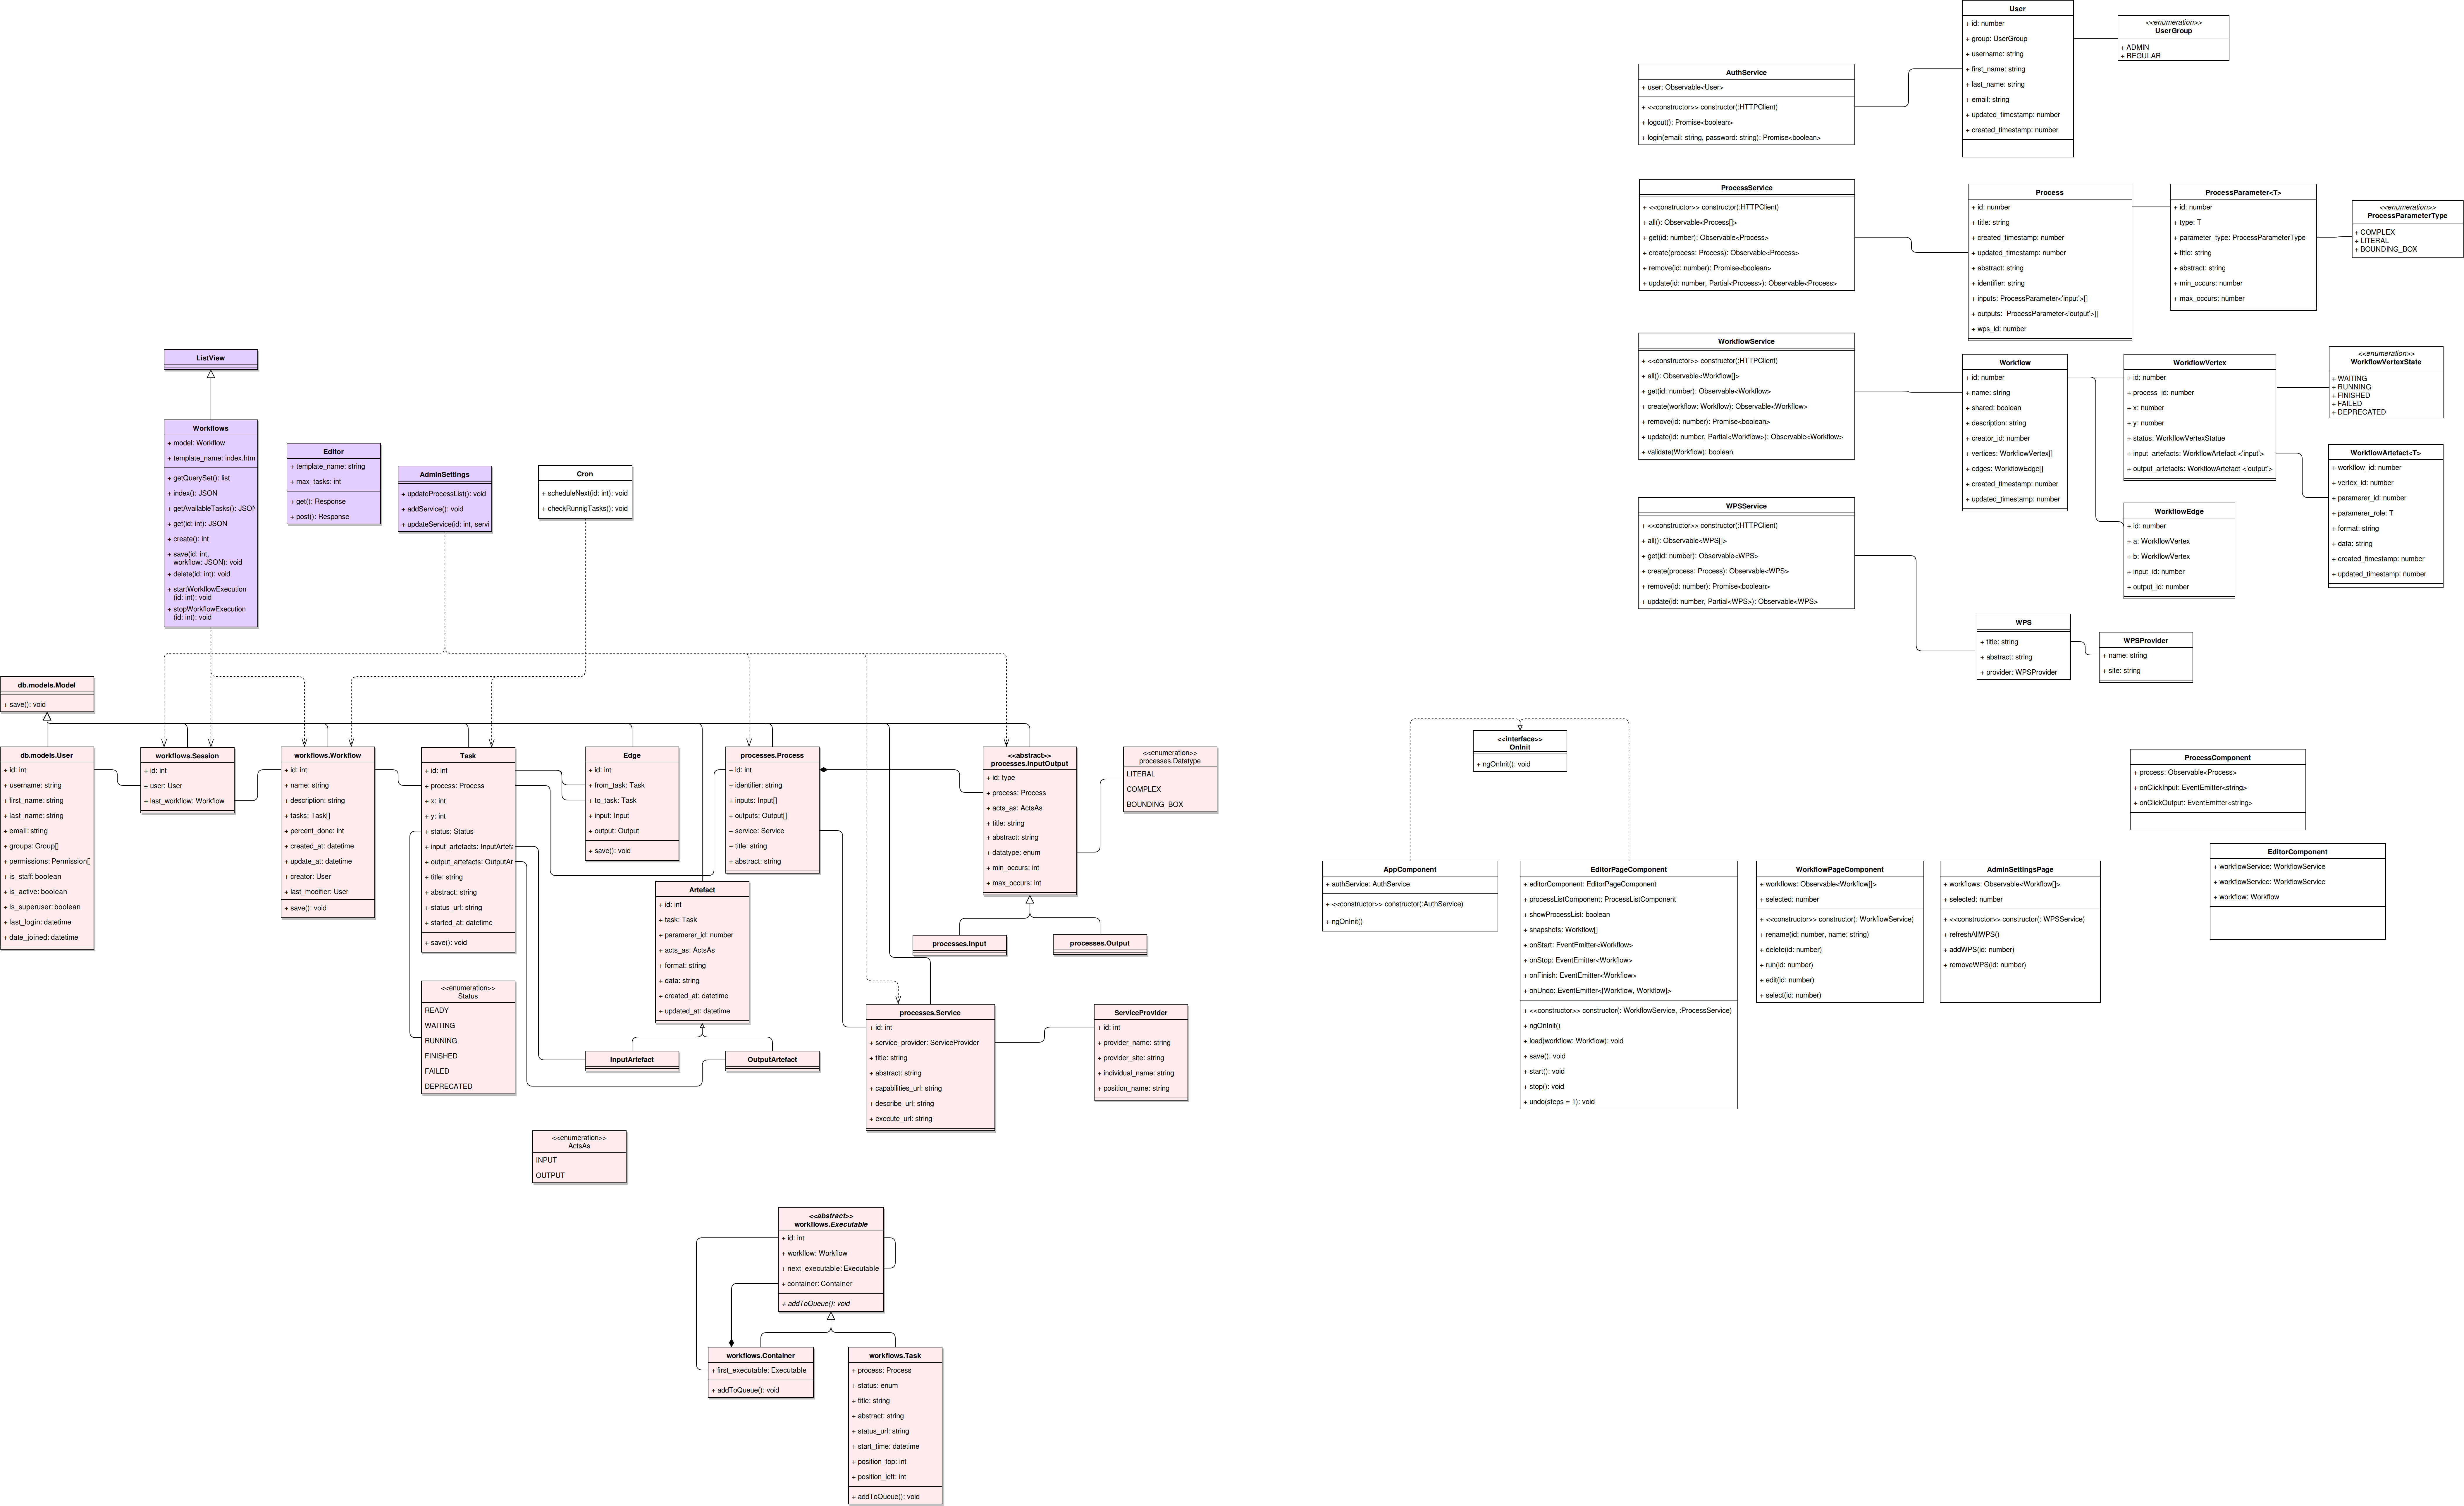
\includegraphics[width=\textwidth]{images/KD.jpg}
	    \caption{Caption}
	    \label{fig:my_label}
	\end{figure}

	
	
	
    \endgroup
	\newpage
	\paperwidth=\pdfpageheight
	\paperheight=\pdfpagewidth
	\pdfpageheight=\paperheight
	\pdfpagewidth=\paperwidth
	\headwidth=\textwidth
	
	\section{test}
	\getlength{\paperwidth}\\
	\getlength{\paperheight}\\
	\getlength{\pdfpageheight}\\
	\getlength{\pdfpagewidth}\\
	\getlength{\headwidth}\\
	\getlength{\footskip}\\
	\getlength{\textwidth}\\
	\getlength{\textheight}\\
	\getlength{\vsize}\\
	\getlength{\hsize}\\